\documentclass[
   % 9b temf, 3b cem?
   accentcolor=9b,
   boxstyle=boxed
   ]{tudasciposter}

% default
\usepackage[ngerman]{babel}
\usepackage{microtype}
\usepackage[autostyle]{csquotes}

% additional
\usepackage{amsmath}
\usepackage{tikz}
\usetikzlibrary{arrows}
\usepackage{pgfplots}
\usepackage{pgfplotstable}
\pgfplotsset{compat=newest}
\usepgfplotslibrary{units}
\usepgfplotslibrary{groupplots}
\usepackage{tuda-pgfplots}

% math font
% option 1
% \usepackage[charter, expert]{mathdesign}
% \usepackage[scaled=.96,osf]{XCharter}% matches the size used in math
% \linespread{1.04}
% option 2
\usepackage[scaled=.98,sups,osf]{XCharter}% lining figures in math, osf in text
\usepackage[scaled=1.04,varqu,varl]{inconsolata}% inconsolata typewriter
\usepackage[type1]{cabin}% sans serif
\usepackage[libertine,vvarbb,scaled=1.05]{newtxmath}
\usepackage[cal=boondoxo]{mathalfa}
\linespread{1.04}
% option 3
% \usepackage[scaled=.98,sups,osf]{XCharter}% lining figures in math, osf in text
% \usepackage[scaled=1.04,varqu,varl]{inconsolata}% inconsolata typewriter
% \usepackage[type1]{cabin}% sans serif
% \usepackage[charter,vvarbb,scaled=1.05]{newtxmath}
% \usepackage[cal=boondoxo]{mathalfa}
% \linespread{1.04}

\begin{document}
\title{Shape Optimization of a Compact DC Photo-Electron Gun using IGA}
\author{Peter Förster$\mathbf{^1}$, Abele Simona$\mathbf{^1}$, Maximilian Herbert$\mathbf{^2}$, Sebastian Schöps$\mathbf{^1}$ and Joachim Enders$\mathbf{^2}$}
\institute{$\mathbf{^1}$ Institut für Teilchenbeschleunigung und Elektromagnetische Felder, TU Darmstadt, $\mathbf{^2}$ Institut für Kernphysik, TU Darmstadt}
\footerqrcode{https://www.temf.tu-darmstadt.de}
\footer{This work is supported by DFG (GRK 2128 ``AccelencE"), BMBF (05H18RDRB1) and DFG (GSC 233)\\

Technische Universität Darmstadt, Institute for Accelerator Science and Electromagnetic Fields, Schloßgartenstr. 8, 64289 Darmstadt, Germany\\
https://www.temf.tu-darmstadt.de}

% temf, temf, ikp
\footergraphics{
   \includegraphics[height=\height]{example-image}
   \includegraphics[height=\height]{example-image}
   \includegraphics[height=\height]{example-image}
}

\begin{tcbposter}[poster={columns=2, rows=20, spacing=1cm}]

\begin{posterboxenv}[title=Motivation]{column=1, row=1, rowspan=8}
   Compact DC photo-electron guns meet the demands of high-current applications such as energy recovery linacs. A main design parameter is the electric field strength, which is limited by the field emission threshold of the electrode material. Optimizing the electrode geometry allows for higher gradients and thus increased gun perfomance.
   \begin{center}
      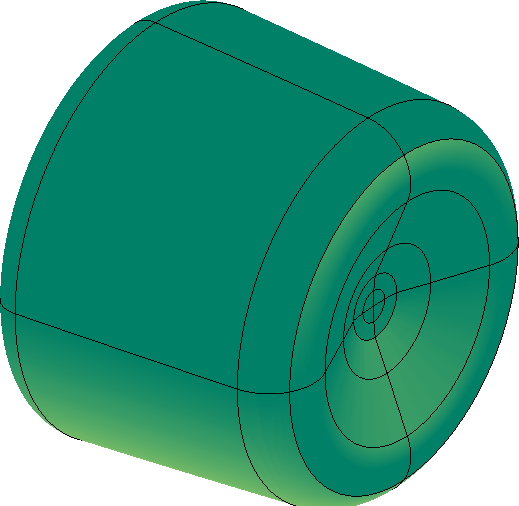
\includegraphics[width=0.35\textwidth]{fig/electrode_init.png}
      \qquad \qquad \qquad
      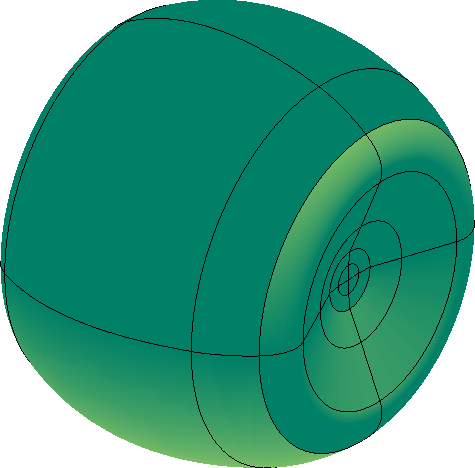
\includegraphics[width=0.35\textwidth]{fig/electrode_opt.png}
   \end{center}
   The problem is described by Maxwell's equations and the PDE for the electrostatic potential reads
   \begin{align*}
      \nabla \cdot (\varepsilon \nabla \varphi) &= 0 \phantom{-00 kV} \quad \mathrm{in}\ \boldsymbol{\Omega},\\
      \varphi &= 0 \phantom{-00 kV} \quad \mathrm{on}\ \boldsymbol{\Gamma}_\mathrm{D_0},\\
      \varphi &= -200\ \mathrm{kV} \quad \mathrm{on}\ \boldsymbol{\Gamma}_\mathrm{D_1},\\
      \partial_n \varphi &= 0 \phantom{-00 kV} \quad \mathrm{on}\ \boldsymbol{\Gamma}_\mathrm{N},
      \end{align*}
   where $\varphi$ is the electrostatic potential, $\varepsilon$ the electric permittivity, $\boldsymbol{\Omega}$ the problem domain and the $\boldsymbol{\Gamma}$'s are the boundaries.
\end{posterboxenv}

\begin{posterboxenv}[title=Isogeometric Analysis]{name=iga, row=9, rowspan=12}
   Isogeometric Analysis employs NURBS basis functions for both the geometry description and as the solution space of the numerical method. This allows to exactly represent curved geometries and at the same time leads to smooth and accurate field solutions.\\

   \begin{center}
      \begin{tikzpicture}[overlay]
   \draw[-, ultra thick] (1, 2.5) to (5, 2.5);
   \draw[-, ultra thick] (5, 2.5) to (5, 6.5);
   \draw[-, ultra thick] (1, 6.5) to (5, 6.5);
   \draw[-, ultra thick] (1, 2.5) to (1, 6.5);

   \draw[-, ultra thick] (1, 3.5) to (5, 3.5);
   \draw[-, ultra thick] (1, 4.5) to (5, 4.5);
   \draw[-, ultra thick] (1, 5.5) to (5, 5.5);
   \draw[-, ultra thick] (2, 2.5) to (2, 6.5);
   \draw[-, ultra thick] (3, 2.5) to (3, 6.5);
   \draw[-, ultra thick] (4, 2.5) to (4, 6.5);

   % coordinate axes
   \draw[->, >=latex, ultra thick] (0, 0) to (1, 0);
   \node[right] at (1, 0) {$\xi$};
   \draw[->, >=latex, ultra thick] (0, 0) to (0, 1);
   \node[above] at (0, 1) {$\eta$};

   \draw[->, ultra thick] (2.5, 0.5) -- (4, 0.5) node[midway, above] {$\Phi$};

   \node at (2.25, 7.5) (o) {$\boldsymbol{\hat{\Omega}}_i$};
   \draw[-, ultra thick] (o.south) -- (2.5, 6);
\end{tikzpicture}

      \hfill
      \begin{tikzpicture}
\begin{axis}[
   scale only axis = true,
   width = 0.9\textwidth,
  axis equal,
  try min ticks=4,
  max space between ticks=1000pt,
  enlargelimits=true,
  colormap/Greens,
  point meta min = 0,
  point meta max = 2,
  x unit=m,
  y unit=m]

  \addplot[surf, shader=interp] table[point meta=\thisrow{c}]{figures/200kV/geometry/geometry_1.dat};

  \addplot[surf, shader=interp] table[point meta=\thisrow{c}]{figures/200kV/geometry/geometry_2.dat};

  \addplot[surf, shader=interp] table[point meta=\thisrow{c}]{figures/200kV/geometry/geometry_3.dat};

  \addplot[surf, shader=interp] table[point meta=\thisrow{c}]{figures/200kV/geometry/geometry_4.dat};

  \addplot[surf, shader=interp] table[point meta=\thisrow{c}]{figures/200kV/geometry/geometry_5.dat};

  \addplot[surf, shader=interp] table[point meta=\thisrow{c}]{figures/200kV/geometry/geometry_6.dat};

  \addplot[surf, shader=interp] table[point meta=\thisrow{c}]{figures/200kV/geometry/geometry_7.dat};

  \addplot[surf, shader=interp] table[point meta=\thisrow{c}]{figures/200kV/geometry/geometry_8.dat};

  \addplot[surf, shader=interp] table[point meta=\thisrow{c}]{figures/200kV/geometry/geometry_9.dat};

  \addplot[surf, shader=interp] table[point meta=\thisrow{c}]{figures/200kV/geometry/geometry_10.dat};

  \addplot[surf, shader=interp] table[point meta=\thisrow{c}]{figures/200kV/geometry/geometry_11.dat};

  \addplot[surf, shader=interp] table[point meta=\thisrow{c}]{figures/200kV/geometry/geometry_12.dat};

  \addplot[surf, shader=interp] table[point meta=\thisrow{c}]{figures/200kV/geometry/geometry_13.dat};

  \addplot[surf, shader=interp, colormap/Reds, point meta min = 0, point meta max = 1] table[point meta=\thisrow{c}]{figures/200kV/geometry/geometry_13.dat};

  \addplot[surf, shader=interp] table[point meta=\thisrow{c}]{figures/200kV/geometry/geometry_14.dat};

  \addplot[surf, shader=interp] table[point meta=\thisrow{c}]{figures/200kV/geometry/geometry_15.dat};

  \addplot[surf, shader=interp, colormap/Reds, point meta min = 0, point meta max = 1] table[point meta=\thisrow{c}]{figures/200kV/geometry/geometry_16.dat};

  \addplot[surf, shader=interp, colormap/Reds, point meta min = 0, point meta max = 1] table[point meta=\thisrow{c}]{figures/200kV/geometry/geometry_17.dat};

  \addplot[surf, shader=interp] table[point meta=\thisrow{c}]{figures/200kV/geometry/geometry_18.dat};

  \addplot[surf, shader=interp] table[point meta=\thisrow{c}]{figures/200kV/geometry/geometry_19.dat};

  \addplot[surf, shader=interp] table[point meta=\thisrow{c}]{figures/200kV/geometry/geometry_20.dat};

  \addplot[surf, shader=interp] table[point meta=\thisrow{c}]{figures/200kV/geometry/geometry_21.dat};

  \addplot[surf, shader=interp] table[point meta=\thisrow{c}]{figures/200kV/geometry/geometry_22.dat};

  % add patch indices
  \addplot[only marks, point meta=explicit symbolic, color=black, nodes near coords] coordinates{
  (0.28,-0.01) [(1)]
  (0.28,-0.005) [(2)]
  (0.28,0.005) [(3)]
  (0.28,0.015) [(4)]
  (0.28,0.045) [(5)]
  (0.24,0.075) [(6)]
  (0.15,0.075) [(7)]
  (0.085,0.075) [(8)]
  (0.1,0.05) [(9)]
  (0.05,0.065) [(10)]
  (0.1,0.04) [(11)]
  (0.05,0.045) [(12)]
  (0.05,0.03) [(13)]
  (0.03,0.0175) [(14)]
  (0.0075,0.0075) [(15)]
  (0.04,0.007) [(16)]
  (0.0075,0.0025) [(17)]
  (0.075,0.017) [(18)]
  (0.115,0.017) [(19)]
  (0.135,0.015) [(20)]
  (0.155,0.025) [(21)]
  (0.035,-0.005) [(22)]
  };

  % add patch boundaries
  \addplot[color=brewerblue] table{figures/200kV/boundary/boundaries11.dat};
  \addplot[color=brewerred] table{figures/200kV/boundary/boundaries12.dat};
  \addplot[color=black] table{figures/200kV/boundary/boundaries13.dat};
  \addplot[color=brewergrey] table{figures/200kV/boundary/boundaries14.dat};

  \addplot[color=brewerblue] table{figures/200kV/boundary/boundaries21.dat};
  \addplot[color=brewerred] table{figures/200kV/boundary/boundaries22.dat};
  \addplot[color=brewergrey] table{figures/200kV/boundary/boundaries23.dat};
  \addplot[color=brewergrey] table{figures/200kV/boundary/boundaries24.dat};

  \addplot[color=brewerblue] table{figures/200kV/boundary/boundaries31.dat};
  \addplot[color=brewerred] table{figures/200kV/boundary/boundaries32.dat};
  \addplot[color=brewergrey] table{figures/200kV/boundary/boundaries33.dat};
  \addplot[color=brewergrey] table{figures/200kV/boundary/boundaries34.dat};

  \addplot[color=brewerblue] table{figures/200kV/boundary/boundaries41.dat};
  \addplot[color=brewerred] table{figures/200kV/boundary/boundaries42.dat};
  \addplot[color=brewergrey] table{figures/200kV/boundary/boundaries43.dat};
  \addplot[color=brewergrey] table{figures/200kV/boundary/boundaries44.dat};

  \addplot[color=brewerblue] table{figures/200kV/boundary/boundaries51.dat};
  \addplot[color=brewerred] table{figures/200kV/boundary/boundaries52.dat};
  \addplot[color=brewergrey] table{figures/200kV/boundary/boundaries53.dat};
  \addplot[color=brewergrey] table{figures/200kV/boundary/boundaries54.dat};

  \addplot[color=brewerblue] table{figures/200kV/boundary/boundaries61.dat};
  \addplot[color=brewerred] table{figures/200kV/boundary/boundaries62.dat};
  \addplot[color=brewergrey] table{figures/200kV/boundary/boundaries63.dat};
  \addplot[color=brewergrey] table{figures/200kV/boundary/boundaries64.dat};

  \addplot[color=brewerblue] table{figures/200kV/boundary/boundaries71.dat};
  \addplot[color=brewerred] table{figures/200kV/boundary/boundaries72.dat};
  \addplot[color=brewergrey] table{figures/200kV/boundary/boundaries73.dat};
  \addplot[color=brewergrey] table{figures/200kV/boundary/boundaries74.dat};

  \addplot[color=brewergrey] table{figures/200kV/boundary/boundaries81.dat};
  \addplot[color=brewerred] table{figures/200kV/boundary/boundaries82.dat};
  \addplot[color=brewergrey] table{figures/200kV/boundary/boundaries83.dat};
  \addplot[color=brewergrey] table{figures/200kV/boundary/boundaries84.dat};

  \addplot[color=brewergrey] table{figures/200kV/boundary/boundaries91.dat};
  \addplot[color=brewerblue] table{figures/200kV/boundary/boundaries92.dat};
  \addplot[color=brewergrey] table{figures/200kV/boundary/boundaries93.dat};
  \addplot[color=brewergrey] table{figures/200kV/boundary/boundaries94.dat};

  \addplot[color=brewerred] table{figures/200kV/boundary/boundaries101.dat};
  \addplot[color=brewergrey] table{figures/200kV/boundary/boundaries102.dat};
  \addplot[color=brewergrey] table{figures/200kV/boundary/boundaries103.dat};
  \addplot[color=brewergrey] table{figures/200kV/boundary/boundaries104.dat};

  \addplot[color=brewergrey] table{figures/200kV/boundary/boundaries111.dat};
  \addplot[color=brewerblue] table{figures/200kV/boundary/boundaries112.dat};
  \addplot[color=brewerblue] table{figures/200kV/boundary/boundaries113.dat};
  \addplot[color=brewergrey] table{figures/200kV/boundary/boundaries114.dat};

  \addplot[color=brewerred] table{figures/200kV/boundary/boundaries121.dat};
  \addplot[color=brewergrey] table{figures/200kV/boundary/boundaries122.dat};
  \addplot[color=brewergrey] table{figures/200kV/boundary/boundaries123.dat};
  \addplot[color=brewergrey] table{figures/200kV/boundary/boundaries124.dat};

  \addplot[color=brewerred] table{figures/200kV/boundary/boundaries131.dat};
  \addplot[color=brewerblue] table{figures/200kV/boundary/boundaries132.dat};
  \addplot[color=brewergrey] table{figures/200kV/boundary/boundaries133.dat};
  \addplot[color=brewergrey] table{figures/200kV/boundary/boundaries134.dat};

  \addplot[color=brewerred] table{figures/200kV/boundary/boundaries141.dat};
  \addplot[color=brewergrey] table{figures/200kV/boundary/boundaries142.dat};
  \addplot[color=brewergrey] table{figures/200kV/boundary/boundaries143.dat};
  \addplot[color=brewergrey] table{figures/200kV/boundary/boundaries144.dat};

  \addplot[color=brewerred] table{figures/200kV/boundary/boundaries151.dat};
  \addplot[color=brewergrey] table{figures/200kV/boundary/boundaries152.dat};
  \addplot[color=brewergrey] table{figures/200kV/boundary/boundaries153.dat};
  \addplot[color=brewergrey] table{figures/200kV/boundary/boundaries154.dat};

  \addplot[color=brewergrey] table{figures/200kV/boundary/boundaries161.dat};
  \addplot[color=brewerblue] table{figures/200kV/boundary/boundaries162.dat};
  \addplot[color=brewergrey] table{figures/200kV/boundary/boundaries163.dat};
  \addplot[color=brewergrey] table{figures/200kV/boundary/boundaries164.dat};

  \addplot[color=brewerred] table{figures/200kV/boundary/boundaries171.dat};
  \addplot[color=brewergrey] table{figures/200kV/boundary/boundaries172.dat};
  \addplot[color=brewergrey] table{figures/200kV/boundary/boundaries173.dat};
  \addplot[color=brewergrey] table{figures/200kV/boundary/boundaries174.dat};

  \addplot[color=brewergrey] table{figures/200kV/boundary/boundaries181.dat};
  \addplot[color=brewergrey] table{figures/200kV/boundary/boundaries182.dat};
  \addplot[color=brewergrey] table{figures/200kV/boundary/boundaries183.dat};
  \addplot[color=brewerblue] table{figures/200kV/boundary/boundaries184.dat};

  \addplot[color=brewergrey] table{figures/200kV/boundary/boundaries191.dat};
  \addplot[color=brewergrey] table{figures/200kV/boundary/boundaries192.dat};
  \addplot[color=brewerblue] table{figures/200kV/boundary/boundaries193.dat};
  \addplot[color=brewerblue] table{figures/200kV/boundary/boundaries194.dat};

  \addplot[color=brewerblue] table{figures/200kV/boundary/boundaries201.dat};
  \addplot[color=brewergrey] table{figures/200kV/boundary/boundaries202.dat};
  \addplot[color=brewerblue] table{figures/200kV/boundary/boundaries203.dat};
  \addplot[color=brewergrey] table{figures/200kV/boundary/boundaries204.dat};

  \addplot[color=brewerblue] table{figures/200kV/boundary/boundaries211.dat};
  \addplot[color=brewerblue] table{figures/200kV/boundary/boundaries212.dat};
  \addplot[color=brewergrey] table{figures/200kV/boundary/boundaries213.dat};
  \addplot[color=brewerblue] table{figures/200kV/boundary/boundaries214.dat};

  \addplot[color=brewerred] table{figures/200kV/boundary/boundaries221.dat};
  \addplot[color=brewerblue] table{figures/200kV/boundary/boundaries222.dat};
  \addplot[color=black] table{figures/200kV/boundary/boundaries223.dat};
  \addplot[color=brewergrey] table{figures/200kV/boundary/boundaries224.dat};
\end{axis}
\end{tikzpicture}

      \begin{tikzpicture}[overlay]
         \draw[->, ultra thick] (-34, 6) to [out=30, in=160] (-22.25, 7.25);
         \draw[->, ultra thick] (-35.75, 3) to [out=20, in=170] (-22, 4.625);
         % coordinate axes
         \draw[->, >=latex, ultra thick] (-32, 0) to (-31, 0);
         \node[right] at (-31, 0) {$x$};
         \draw[->, >=latex, ultra thick] (-32, 0) to (-32, 1);
         \node[above] at (-32, 1) {$y$};

         \node at (-20, 7.5) (o) {$\boldsymbol{\Omega}_i$};
         \draw[-, ultra thick] (o.west) -- (-21.5, 7);
      \end{tikzpicture}
   \end{center}

   Due to the axisymmetry of the geometry it suffices to consider half of the longitudinal cross-section of the gun.
   The elements of any patch $i$ share a single parameter space $\boldsymbol{\hat{\Omega}}_i$ and are mapped to the physical space $\boldsymbol{\Omega}_i$ via a NURBS mapping
   \begin{align*}
      \Phi\colon \boldsymbol{\hat{\Omega}}_i &\to \boldsymbol{\Omega}_i\\
      (\eta, \xi) &\mapsto (x, y).
   \end{align*}

   \begin{center}
      \begin{tikzpicture}

   \draw[->, >=latex, ultra thick] (1, 12) to (2, 12);
   \node[right] at (2, 12) {$x$};
   \draw[->, >=latex, ultra thick] (1, 12) to (1, 13);
   \node[above] at (1, 13) {$y$};

\begin{axis}[
   scale only axis=true,
   width=\textwidth,
   axis equal,
   try min ticks=4,
   max space between ticks=1000pt,
   enlargelimits=true,
   x unit=m,
   y unit=m,
   legend entries={$C^1$-NURBS, Original Control Points, Control Polygon},
   legend style={at={(0.75, 0.75)}, anchor=north west, draw=none},
   hide axis
   ]

   \addplot[color=black, ultra thick] table {fig/nurbs-init/nurbs_5_1.dat};
   \addplot[color=TUDa-9a, mark=*, only marks, mark size=6] table {fig/nurbs-init/nurbs_5_1_coefs.dat};
   \addplot[color=TUDa-0b, dashed, ultra thick] table {fig/nurbs-init/nurbs_5_1_net.dat};

   \addplot[color=black, ultra thick] table {fig/nurbs-init/nurbs_6_3.dat};
   \addplot[color=TUDa-9a, mark=*, only marks, mark size=6] table {fig/nurbs-init/nurbs_6_3_coefs.dat};
   \addplot[color=TUDa-0b, dashed, ultra thick] table {fig/nurbs-init/nurbs_6_3_net.dat};

   \addplot[color=black, ultra thick] table {fig/nurbs-init/nurbs_7_3.dat};
   \addplot[color=TUDa-9a, mark=*, only marks, mark size=6] table {fig/nurbs-init/nurbs_7_3_coefs.dat};
   \addplot[color=TUDa-0b, dashed, ultra thick] table {fig/nurbs-init/nurbs_7_3_net.dat};

   \addplot[color=black, ultra thick] table {fig/nurbs-init/nurbs_8_3.dat};
   \addplot[color=TUDa-9a, mark=*, only marks, mark size=6] table {fig/nurbs-init/nurbs_8_3_coefs.dat};
   \addplot[color=TUDa-0b, dashed, ultra thick] table {fig/nurbs-init/nurbs_8_3_net.dat};

   \addplot[color=black, ultra thick] table {fig/nurbs-init/nurbs_9_2.dat};
   \addplot[color=TUDa-9a, mark=*, only marks, mark size=6] table {fig/nurbs-init/nurbs_9_2_coefs.dat};
   \addplot[color=TUDa-0b, dashed, ultra thick] table {fig/nurbs-init/nurbs_9_2_net.dat};

\end{axis}

   \draw[<->, >=latex', ultra thick] (3, 11) to (33.5, 11);
   \node at (18.25, 10) {$102$ mm};
   \draw[<->, >=latex', ultra thick] (2, 14) to (2, 20.5);
   \node[rotate=90] at (1, 17.25) {$20$ mm};

\end{tikzpicture}

   \end{center}

   Individual curves can easily be manipulated by moving their control points and multiple curves may be glued together to attain higher continuity across their interfaces.
   Using the above $C^1$-continuous curve for the optimization guarantees an optimized geometry that fulfills manufacturing requirements.
\end{posterboxenv}

\begin{posterboxenv}[title=Shape Optimization]{name=geo, column=2, row=1, rowspan=9}
   The aim of the optimization is to minimize the maximal electric field strength in the vicinity of the electrode. This is accomplished by finding an optimal configuration of the control points under additional geometric constraints.
   The cost function is given by
   \begin{align*}
      f(\mathbf{p}) = \frac{1}{|I|} \sum_{i \in I} \max_{\mathbf{x} \in \boldsymbol{\Omega}_i} \Vert \mathbf{E}(\mathbf{x}) \Vert_2,
   \end{align*}
   where $\mathbf{p}$ is a vector containing the control point coordinates, $I$ is an index set and $\mathbf{E}$ is the electric field. The maxima are averaged to ensure that the field strength is simultaneously minimized across all patches.
   The full optimization problem then reads
   \begin{align*}
      \min_\mathbf{p}& \quad f(\mathbf{p}),\\
      \mathrm{subject\ to}& \quad \mathbf{h}(\mathbf{p}) \leq \mathbf{0},
   \end{align*}
   where $\mathbf{h}$ is made up of constraints on the volume of the electrode and the relative position of the control points.

   \begin{center}
      \begin{tikzpicture}[scale=1]
\begin{axis}[
   scale only axis = true,
   width = 0.45\textwidth,
   axis equal,
   try min ticks=4,
   max space between ticks=1000pt,
   enlargelimits=true,
   x unit=m,
   y unit=m,
   hide axis]

   \addplot[color=black] table {nurbs-opt/nurbs_5_1.dat};
   \addplot[color=TUDa-9a, mark=*, only marks] table {nurbs-opt/nurbs_5_1_coefs.dat};
   \addplot[color=TUDa-0b, dashed] table {nurbs-opt/nurbs_5_1_net.dat};

   \addplot[color=black] table {nurbs-opt/nurbs_6_3.dat};
   \addplot[color=TUDa-9a, mark=*, only marks] table {nurbs-opt/nurbs_6_3_coefs.dat};
   \addplot[color=TUDa-0b, dashed] table {nurbs-opt/nurbs_6_3_net.dat};

   \addplot[color=black] table {nurbs-opt/nurbs_7_3.dat};
   \addplot[color=TUDa-9a, mark=*, only marks] table {nurbs-opt/nurbs_7_3_coefs.dat};
   \addplot[color=TUDa-0b, dashed] table {nurbs-opt/nurbs_7_3_net.dat};

   \addplot[color=black] table {nurbs-opt/nurbs_8_3.dat};
   \addplot[color=TUDa-9a, mark=*, only marks] table {nurbs-opt/nurbs_8_3_coefs.dat};
   \addplot[color=TUDa-0b, dashed] table {nurbs-opt/nurbs_8_3_net.dat};

   \addplot[color=black] table {nurbs-opt/nurbs_9_2.dat};
   \addplot[color=TUDa-9a, mark=*, only marks] table {nurbs-opt/nurbs_9_2_coefs.dat};
   \addplot[color=TUDa-0b, dashed] table {nurbs-opt/nurbs_9_2_net.dat};
\end{axis}
\end{tikzpicture}

   \end{center}
\end{posterboxenv}


\begin{posterboxenv}[title=Results]{name=res, column=2, row=10, rowspan=11}
   The results show the magnitude of the eletric field in the region of interest. A significant improvement in terms of the maximal value is visible.
   Originally we had $\max_{\mathbf{x} \in \boldsymbol{\Omega}_i} \Vert \mathbf{E}(\mathbf{x}) \Vert_2 = \mathbf{7.62}\ \mathrm{MVm^{-1}}$ and after optimization we obtained $\max_{\mathbf{x} \in \boldsymbol{\Omega}_i} \Vert \mathbf{E}(\mathbf{x}) \Vert_2 = \mathbf{5.837}\ \mathrm{MVm^{-1}}$.\\

   \begin{center}
      \begin{tikzpicture}

\begin{axis}[
   scale only axis=true,
   width=\textwidth,
   axis equal,
   try min ticks=4,
   max space between ticks=1000pt,
   enlargelimits=true,
   colormap name=tuda,
   point meta min=0,
   point meta max=10e6,
   colorbar,
   colorbar style={at={(1, 0.65)}, anchor=north west, height=0.3*\pgfkeysvalueof{/pgfplots/parent axis height}, ytick={0, 0.2e7, 0.4e7, 0.6e7, 0.8e7, 1e7}},
   hide axis]

  % \addplot[surf, shader=faceted interp] table[point meta=\thisrow{c}]{fig/v5_order=3/init_degree=3_nsub=128/E_degree=3_nsub=128_1.dat};
  %
  % \addplot[surf, shader=faceted interp] table[point meta=\thisrow{c}]{fig/v5_order=3/init_degree=3_nsub=128/E_degree=3_nsub=128_2.dat};
  %
  % \addplot[surf, shader=faceted interp] table[point meta=\thisrow{c}]{fig/v5_order=3/init_degree=3_nsub=128/E_degree=3_nsub=128_3.dat};
  %
  % \addplot[surf, shader=faceted interp] table[point meta=\thisrow{c}]{fig/v5_order=3/init_degree=3_nsub=128/E_degree=3_nsub=128_4.dat};
  %
  % \addplot[surf, shader=faceted interp] table{fig/v5_order=3/init_degree=3_nsub=128/E_degree=3_nsub=128_5.dat};

  \addplot[surf, shader=faceted interp] table[point meta=\thisrow{c}]{fig/v5_order=3/init_degree=3_nsub=128/E_degree=3_nsub=128_6.dat};

  \addplot[surf, shader=faceted interp] table[point meta=\thisrow{c}]{fig/v5_order=3/init_degree=3_nsub=128/E_degree=3_nsub=128_7.dat};

  \addplot[surf, shader=faceted interp] table[point meta=\thisrow{c}]{fig/v5_order=3/init_degree=3_nsub=128/E_degree=3_nsub=128_8.dat};

  \addplot[surf, shader=faceted interp] table[point meta=\thisrow{c}]{fig/v5_order=3/init_degree=3_nsub=128/E_degree=3_nsub=128_9.dat};

  % \addplot[surf, shader=faceted interp] table[point meta=\thisrow{c}]{fig/v5_order=3/init_degree=3_nsub=128/E_degree=3_nsub=128_10.dat};
  %
  % \addplot[surf, shader=faceted interp] table[point meta=\thisrow{c}]{fig/v5_order=3/init_degree=3_nsub=128/E_degree=3_nsub=128_11.dat};
  %
  % \addplot[surf, shader=faceted interp] table[point meta=\thisrow{c}]{fig/v5_order=3/init_degree=3_nsub=128/E_degree=3_nsub=128_12.dat};
  %
  % \addplot[surf, shader=faceted interp] table[point meta=\thisrow{c}]{fig/v5_order=3/init_degree=3_nsub=128/E_degree=3_nsub=128_13.dat};
  %
  % \addplot[surf, shader=faceted interp] table[point meta=\thisrow{c}]{fig/v5_order=3/init_degree=3_nsub=128/E_degree=3_nsub=128_13.dat};
  %
  % \addplot[surf, shader=faceted interp] table[point meta=\thisrow{c}]{fig/v5_order=3/init_degree=3_nsub=128/E_degree=3_nsub=128_14.dat};
  %
  % \addplot[surf, shader=faceted interp] table[point meta=\thisrow{c}]{fig/v5_order=3/init_degree=3_nsub=128/E_degree=3_nsub=128_15.dat};

  % \addplot[surf, shader=faceted interp] table[point meta=\thisrow{c}]{fig/v5_order=3/init_degree=3_nsub=128/E_degree=3_nsub=128_128.dat};
  %
  % \addplot[surf, shader=faceted interp] table[point meta=\thisrow{c}]{fig/v5_order=3/init_degree=3_nsub=128/E_degree=3_nsub=128_17.dat};

  % \addplot[surf, shader=faceted interp] table[point meta=\thisrow{c}]{fig/v5_order=3/init_degree=3_nsub=128/E_degree=3_nsub=128_18.dat};
  %
  % \addplot[surf, shader=faceted interp] table[point meta=\thisrow{c}]{fig/v5_order=3/init_degree=3_nsub=128/E_degree=3_nsub=128_19.dat};
  %
  % \addplot[surf, shader=faceted interp] table[point meta=\thisrow{c}]{fig/v5_order=3/init_degree=3_nsub=128/E_degree=3_nsub=128_20.dat};
  %
  % \addplot[surf, shader=faceted interp] table[point meta=\thisrow{c}]{fig/v5_order=3/init_degree=3_nsub=128/E_degree=3_nsub=128_21.dat};
  %
  % \addplot[surf, shader=faceted interp] table[point meta=\thisrow{c}]{fig/v5_order=3/init_degree=3_nsub=128/E_degree=3_nsub=128_22.dat};
  %
  % \addplot[surf, shader=faceted interp] table[point meta=\thisrow{c}]{fig/v5_order=3/init_degree=3_nsub=128/E_degree=3_nsub=128_23.dat};
  %
  % \addplot[surf, shader=faceted interp] table[point meta=\thisrow{c}]{fig/v5_order=3/init_degree=3_nsub=128/E_degree=3_nsub=128_24.dat};
  %
  % \addplot[surf, shader=faceted interp] table[point meta=\thisrow{c}]{fig/v5_order=3/init_degree=3_nsub=128/E_degree=3_nsub=128_25.dat};

  % \addplot[color=TUDa-2a, ultra thick] table{fig/geometry/boundary11.dat};
  % \addplot[color=TUDa-9a, ultra thick] table{fig/geometry/boundary12.dat};
  % \addplot[color=black, ultra thick] table{fig/geometry/boundary13.dat};
  % \addplot[color=TUDa-0b, ultra thick] table{fig/geometry/boundary14.dat};
  %
  % \addplot[color=TUDa-2a, ultra thick] table{fig/geometry/boundary21.dat};
  % \addplot[color=TUDa-9a, ultra thick] table{fig/geometry/boundary22.dat};
  % \addplot[color=TUDa-0b, ultra thick] table{fig/geometry/boundary23.dat};
  % \addplot[color=TUDa-0b, ultra thick] table{fig/geometry/boundary24.dat};
  %
  % \addplot[color=TUDa-2a, ultra thick] table{fig/geometry/boundary31.dat};
  % \addplot[color=TUDa-9a, ultra thick] table{fig/geometry/boundary32.dat};
  % \addplot[color=TUDa-0b, ultra thick] table{fig/geometry/boundary33.dat};
  % \addplot[color=TUDa-0b, ultra thick] table{fig/geometry/boundary34.dat};
  %
  % \addplot[color=TUDa-2a, ultra thick] table{fig/geometry/boundary41.dat};
  % \addplot[color=TUDa-9a, ultra thick] table{fig/geometry/boundary42.dat};
  % \addplot[color=TUDa-0b, ultra thick] table{fig/geometry/boundary43.dat};
  % \addplot[color=TUDa-0b, ultra thick] table{fig/geometry/boundary44.dat};

  % \addplot[color=TUDa-2a, ultra thick] table{fig/geometry/boundary51.dat};
  % \addplot[color=TUDa-9a, ultra thick] table{fig/geometry/boundary52.dat};
  % \addplot[color=TUDa-0b, ultra thick] table{fig/geometry/boundary53.dat};
  % \addplot[color=TUDa-0b, ultra thick] table{fig/geometry/boundary54.dat};
  %
  % \addplot[color=TUDa-0b, ultra thick] table{fig/geometry/boundary61.dat};
  % \addplot[color=TUDa-0b, ultra thick] table{fig/geometry/boundary62.dat};
  % \addplot[color=TUDa-2a, ultra thick] table{fig/geometry/boundary63.dat};
  % \addplot[color=TUDa-9a, ultra thick] table{fig/geometry/boundary64.dat};
  %
  % \addplot[color=TUDa-0b, ultra thick] table{fig/geometry/boundary71.dat};
  % \addplot[color=TUDa-0b, ultra thick] table{fig/geometry/boundary72.dat};
  % \addplot[color=TUDa-2a, ultra thick] table{fig/geometry/boundary73.dat};
  % \addplot[color=TUDa-9a, ultra thick] table{fig/geometry/boundary74.dat};
  %
  % \addplot[color=TUDa-0b, ultra thick] table{fig/geometry/boundary81.dat};
  % \addplot[color=TUDa-0b, ultra thick] table{fig/geometry/boundary82.dat};
  % \addplot[color=TUDa-2a, ultra thick] table{fig/geometry/boundary83.dat};
  % \addplot[color=TUDa-0b, ultra thick] table{fig/geometry/boundary84.dat};
  %
  % \addplot[color=TUDa-0b, ultra thick] table{fig/geometry/boundary91.dat};
  % \addplot[color=TUDa-2a, ultra thick] table{fig/geometry/boundary92.dat};
  % \addplot[color=TUDa-2a, ultra thick] table{fig/geometry/boundary93.dat};
  % \addplot[color=TUDa-0b, ultra thick] table{fig/geometry/boundary94.dat};

  % \addplot[color=TUDa-9a, ultra thick] table{fig/geometry/boundary101.dat};
  % \addplot[color=TUDa-0b, ultra thick] table{fig/geometry/boundary102.dat};
  % \addplot[color=TUDa-0b, ultra thick] table{fig/geometry/boundary103.dat};
  % \addplot[color=TUDa-9a, ultra thick] table{fig/geometry/boundary104.dat};
  %
  % \addplot[color=TUDa-9a, ultra thick] table{fig/geometry/boundary111.dat};
  % \addplot[color=TUDa-0b, ultra thick] table{fig/geometry/boundary112.dat};
  % \addplot[color=TUDa-0b, ultra thick] table{fig/geometry/boundary113.dat};
  % \addplot[color=TUDa-0b, ultra thick] table{fig/geometry/boundary114.dat};
  %
  % \addplot[color=TUDa-9a, ultra thick] table{fig/geometry/boundary121.dat};
  % \addplot[color=TUDa-2a, ultra thick] table{fig/geometry/boundary122.dat};
  % \addplot[color=TUDa-0b, ultra thick] table{fig/geometry/boundary123.dat};
  % \addplot[color=TUDa-0b, ultra thick] table{fig/geometry/boundary124.dat};
  %
  % \addplot[color=TUDa-9a, ultra thick] table{fig/geometry/boundary131.dat};
  % \addplot[color=TUDa-0b, ultra thick] table{fig/geometry/boundary132.dat};
  % \addplot[color=TUDa-0b, ultra thick] table{fig/geometry/boundary133.dat};
  % \addplot[color=TUDa-0b, ultra thick] table{fig/geometry/boundary134.dat};
  %
  % \addplot[color=TUDa-0b, ultra thick] table{fig/geometry/boundary141.dat};
  % \addplot[color=TUDa-0b, ultra thick] table{fig/geometry/boundary142.dat};
  % \addplot[color=TUDa-0b, ultra thick] table{fig/geometry/boundary143.dat};
  % \addplot[color=TUDa-2a, ultra thick] table{fig/geometry/boundary144.dat};
  %
  % \addplot[color=TUDa-9a, ultra thick] table{fig/geometry/boundary151.dat};
  % \addplot[color=TUDa-9a, ultra thick] table{fig/geometry/boundary152.dat};
  % \addplot[color=TUDa-9a, ultra thick] table{fig/geometry/boundary153.dat};
  % \addplot[color=TUDa-0b, ultra thick] table{fig/geometry/boundary154.dat};
  %
  % % \addplot[color=TUDa-0b, ultra thick] table{fig/geometry/boundary161.dat};
  % % \addplot[color=TUDa-0b, ultra thick] table{fig/geometry/boundary162.dat};
  % \addplot[color=TUDa-9a, ultra thick] table{fig/geometry/boundary163.dat};
  % \addplot[color=TUDa-9a, ultra thick] table{fig/geometry/boundary164.dat};
  %
  % % \addplot[color=TUDa-0b, ultra thick] table{fig/geometry/boundary171.dat};
  % \addplot[color=TUDa-9a, ultra thick] table{fig/geometry/boundary172.dat};
  % \addplot[color=TUDa-9a, ultra thick] table{fig/geometry/boundary173.dat};
  % \addplot[color=TUDa-9a, ultra thick] table{fig/geometry/boundary174.dat};
  %
  % \addplot[color=TUDa-9a, ultra thick] table{fig/geometry/boundary181.dat};
  % \addplot[color=TUDa-2a, ultra thick] table{fig/geometry/boundary182.dat};
  % \addplot[color=TUDa-0b, ultra thick] table{fig/geometry/boundary183.dat};
  % \addplot[color=TUDa-0b, ultra thick] table{fig/geometry/boundary184.dat};
  %
  % \addplot[color=TUDa-9a, ultra thick] table{fig/geometry/boundary191.dat};
  % \addplot[color=TUDa-0b, ultra thick] table{fig/geometry/boundary192.dat};
  % \addplot[color=black, ultra thick] table{fig/geometry/boundary193.dat};
  % \addplot[color=TUDa-9a, ultra thick] table{fig/geometry/boundary194.dat};
  %
  % \addplot[color=TUDa-0b, ultra thick] table{fig/geometry/boundary201.dat};
  % \addplot[color=TUDa-0b, ultra thick] table{fig/geometry/boundary202.dat};
  % \addplot[color=black, ultra thick] table{fig/geometry/boundary203.dat};
  % \addplot[color=TUDa-9a, ultra thick] table{fig/geometry/boundary204.dat};
  %
  % \addplot[color=TUDa-0b, ultra thick] table{fig/geometry/boundary211.dat};
  % \addplot[color=TUDa-2a, ultra thick] table{fig/geometry/boundary212.dat};
  % \addplot[color=black, ultra thick] table{fig/geometry/boundary213.dat};
  % \addplot[color=TUDa-0b, ultra thick] table{fig/geometry/boundary214.dat};
  %
  % \addplot[color=TUDa-0b, ultra thick] table{fig/geometry/boundary221.dat};
  % \addplot[color=TUDa-0b, ultra thick] table{fig/geometry/boundary222.dat};
  % \addplot[color=TUDa-2a, ultra thick] table{fig/geometry/boundary223.dat};
  % \addplot[color=TUDa-2a, ultra thick] table{fig/geometry/boundary224.dat};
  %
  % \addplot[color=TUDa-2a, ultra thick] table{fig/geometry/boundary231.dat};
  % \addplot[color=TUDa-2a, ultra thick] table{fig/geometry/boundary232.dat};
  % \addplot[color=TUDa-2a, ultra thick] table{fig/geometry/boundary233.dat};
  % \addplot[color=TUDa-0b, ultra thick] table{fig/geometry/boundary234.dat};
  %
  % \addplot[color=TUDa-0b, ultra thick] table{fig/geometry/boundary241.dat};
  % \addplot[color=TUDa-2a, ultra thick] table{fig/geometry/boundary242.dat};
  % \addplot[color=TUDa-0b, ultra thick] table{fig/geometry/boundary243.dat};
  % \addplot[color=TUDa-0b, ultra thick] table{fig/geometry/boundary244.dat};
  %
  % \addplot[color=TUDa-2a, ultra thick] table{fig/geometry/boundary251.dat};
  % \addplot[color=TUDa-2a, ultra thick] table{fig/geometry/boundary252.dat};
  % \addplot[color=TUDa-0b, ultra thick] table{fig/geometry/boundary253.dat};
  % \addplot[color=TUDa-2a, ultra thick] table{fig/geometry/boundary254.dat};

\end{axis}

\end{tikzpicture}


      \begin{tikzpicture}

\begin{axis}[
   % scale only axis=true,
   width=\textwidth,
   axis equal,
   % xmin=0.05,
   % xmax=0.4,
   % ymin=0,
   % ymax=0.13,
   try min ticks=4,
   max space between ticks=1000pt,
   % enlargelimits=true,
   colormap name=tuda,
   point meta min=0,
   point meta max=10e6,
   colorbar,
   colorbar style={at={(1, 0.65)}, anchor=north west, height=0.3*\pgfkeysvalueof{/pgfplots/parent axis height}, ytick={0, 0.2e7, 0.4e7, 0.6e7, 0.8e7, 1e7}, ylabel=$\Vert \mathbf{E} \Vert_2$ / $\mathrm{Vm}^{-1}$},
   hide axis
   ]

  % \addplot[surf, shader=faceted interp] table[point meta=\thisrow{c}]{fig/v5_order=3/run18_degree=3_nsub=128/E_degree=3_nsub=128_1.dat};
  %
  % \addplot[surf, shader=faceted interp] table[point meta=\thisrow{c}]{fig/v5_order=3/run18_degree=3_nsub=128/E_degree=3_nsub=128_2.dat};
  %
  % \addplot[surf, shader=faceted interp] table[point meta=\thisrow{c}]{fig/v5_order=3/run18_degree=3_nsub=128/E_degree=3_nsub=128_3.dat};
  %
  % \addplot[surf, shader=faceted interp] table[point meta=\thisrow{c}]{fig/v5_order=3/run18_degree=3_nsub=128/E_degree=3_nsub=128_4.dat};
  %
  % \addplot[surf, shader=faceted interp] table[point meta=\thisrow{c}]{fig/v5_order=3/run18_degree=3_nsub=128/E_degree=3_nsub=128_5.dat};

  \addplot[surf, shader=faceted interp] table[point meta=\thisrow{c}]{fig/v5_order=3/run18_degree=3_nsub=128/E_degree=3_nsub=128_6.dat};

  \addplot[surf, shader=faceted interp] table[point meta=\thisrow{c}]{fig/v5_order=3/run18_degree=3_nsub=128/E_degree=3_nsub=128_7.dat};

  \addplot[surf, shader=faceted interp] table[point meta=\thisrow{c}]{fig/v5_order=3/run18_degree=3_nsub=128/E_degree=3_nsub=128_8.dat};

  \addplot[surf, shader=faceted interp] table[point meta=\thisrow{c}]{fig/v5_order=3/run18_degree=3_nsub=128/E_degree=3_nsub=128_9.dat};

  % \addplot[surf, shader=faceted interp] table[point meta=\thisrow{c}]{fig/v5_order=3/run18_degree=3_nsub=128/E_degree=3_nsub=128_10.dat};
  %
  % \addplot[surf, shader=faceted interp] table[point meta=\thisrow{c}]{fig/v5_order=3/run18_degree=3_nsub=128/E_degree=3_nsub=128_11.dat};
  %
  % \addplot[surf, shader=interp] table[point meta=\thisrow{c}]{fig/v5_order=3/run18_degree=3_nsub=128/E_degree=3_nsub=128_12.dat};
  %
  % \addplot[surf, shader=interp] table[point meta=\thisrow{c}]{fig/v5_order=3/run18_degree=3_nsub=128/E_degree=3_nsub=128_13.dat};
  %
  % \addplot[surf, shader=interp] table[point meta=\thisrow{c}]{fig/v5_order=3/run18_degree=3_nsub=128/E_degree=3_nsub=128_13.dat};
  %
  % \addplot[surf, shader=interp] table[point meta=\thisrow{c}]{fig/v5_order=3/run18_degree=3_nsub=128/E_degree=3_nsub=128_14.dat};
  %
  % \addplot[surf, shader=interp] table[point meta=\thisrow{c}]{fig/v5_order=3/run18_degree=3_nsub=128/E_degree=3_nsub=128_15.dat};
  %
  % \addplot[surf, shader=interp] table[point meta=\thisrow{c}]{fig/v5_order=3/run18_degree=3_nsub=128/E_degree=3_nsub=128_16.dat};
  %
  % \addplot[surf, shader=interp] table[point meta=\thisrow{c}]{fig/v5_order=3/run18_degree=3_nsub=128/E_degree=3_nsub=128_17.dat};
  %
  % \addplot[surf, shader=interp] table[point meta=\thisrow{c}]{fig/v5_order=3/run18_degree=3_nsub=128/E_degree=3_nsub=128_18.dat};
  %
  % \addplot[surf, shader=interp] table[point meta=\thisrow{c}]{fig/v5_order=3/run18_degree=3_nsub=128/E_degree=3_nsub=128_19.dat};
  %
  % \addplot[surf, shader=interp] table[point meta=\thisrow{c}]{fig/v5_order=3/run18_degree=3_nsub=128/E_degree=3_nsub=128_20.dat};
  %
  % \addplot[surf, shader=interp] table[point meta=\thisrow{c}]{fig/v5_order=3/run18_degree=3_nsub=128/E_degree=3_nsub=128_21.dat};
  %
  % \addplot[surf, shader=interp] table[point meta=\thisrow{c}]{fig/v5_order=3/run18_degree=3_nsub=128/E_degree=3_nsub=128_22.dat};
  %
  % \addplot[surf, shader=interp] table[point meta=\thisrow{c}]{fig/v5_order=3/run18_degree=3_nsub=128/E_degree=3_nsub=128_23.dat};
  %
  % \addplot[surf, shader=interp] table[point meta=\thisrow{c}]{fig/v5_order=3/run18_degree=3_nsub=128/E_degree=3_nsub=128_24.dat};
  %
  % \addplot[surf, shader=interp] table[point meta=\thisrow{c}]{fig/v5_order=3/run18_degree=3_nsub=128/E_degree=3_nsub=128_25.dat};

  % \addplot[color=TUDa-2a, ultra thick] table{fig/geometry/boundary11.dat};
  % \addplot[color=TUDa-9a, ultra thick] table{fig/geometry/boundary12.dat};
  % \addplot[color=black, ultra thick] table{fig/geometry/boundary13.dat};
  % \addplot[color=TUDa-0b, ultra thick] table{fig/geometry/boundary14.dat};
  %
  % \addplot[color=TUDa-2a, ultra thick] table{fig/geometry/boundary21.dat};
  % \addplot[color=TUDa-9a, ultra thick] table{fig/geometry/boundary22.dat};
  % \addplot[color=TUDa-0b, ultra thick] table{fig/geometry/boundary23.dat};
  % \addplot[color=TUDa-0b, ultra thick] table{fig/geometry/boundary24.dat};
  %
  % \addplot[color=TUDa-2a, ultra thick] table{fig/geometry/boundary31.dat};
  % \addplot[color=TUDa-9a, ultra thick] table{fig/geometry/boundary32.dat};
  % \addplot[color=TUDa-0b, ultra thick] table{fig/geometry/boundary33.dat};
  % \addplot[color=TUDa-0b, ultra thick] table{fig/geometry/boundary34.dat};
  %
  % \addplot[color=TUDa-2a, ultra thick] table{fig/geometry/boundary41.dat};
  % \addplot[color=TUDa-9a, ultra thick] table{fig/geometry/boundary42.dat};
  % \addplot[color=TUDa-0b, ultra thick] table{fig/geometry/boundary43.dat};
  % \addplot[color=TUDa-0b, ultra thick] table{fig/geometry/boundary44.dat};

  % \addplot[color=TUDa-2a, ultra thick] table{fig/geometry/boundary51.dat};
  % \addplot[color=TUDa-9a, ultra thick] table{fig/geometry/boundary52.dat};
  % \addplot[color=TUDa-0b, ultra thick] table{fig/geometry/boundary53.dat};
  % \addplot[color=TUDa-0b, ultra thick] table{fig/geometry/boundary54.dat};
  %
  % \addplot[color=TUDa-0b, ultra thick] table{fig/geometry/boundary61.dat};
  % \addplot[color=TUDa-0b, ultra thick] table{fig/geometry/boundary62.dat};
  % \addplot[color=TUDa-2a, ultra thick] table{fig/geometry/boundary63.dat};
  % \addplot[color=TUDa-9a, ultra thick] table{fig/geometry/boundary64.dat};
  %
  % \addplot[color=TUDa-0b, ultra thick] table{fig/geometry/boundary71.dat};
  % \addplot[color=TUDa-0b, ultra thick] table{fig/geometry/boundary72.dat};
  % \addplot[color=TUDa-2a, ultra thick] table{fig/geometry/boundary73.dat};
  % \addplot[color=TUDa-9a, ultra thick] table{fig/geometry/boundary74.dat};
  %
  % \addplot[color=TUDa-0b, ultra thick] table{fig/geometry/boundary81.dat};
  % \addplot[color=TUDa-0b, ultra thick] table{fig/geometry/boundary82.dat};
  % \addplot[color=TUDa-2a, ultra thick] table{fig/geometry/boundary83.dat};
  % \addplot[color=TUDa-0b, ultra thick] table{fig/geometry/boundary84.dat};
  %
  % \addplot[color=TUDa-0b, ultra thick] table{fig/geometry/boundary91.dat};
  % \addplot[color=TUDa-2a, ultra thick] table{fig/geometry/boundary92.dat};
  % \addplot[color=TUDa-2a, ultra thick] table{fig/geometry/boundary93.dat};
  % \addplot[color=TUDa-0b, ultra thick] table{fig/geometry/boundary94.dat};

  % \addplot[color=TUDa-9a, ultra thick] table{fig/geometry/boundary101.dat};
  % \addplot[color=TUDa-0b, ultra thick] table{fig/geometry/boundary102.dat};
  % \addplot[color=TUDa-0b, ultra thick] table{fig/geometry/boundary103.dat};
  % \addplot[color=TUDa-9a, ultra thick] table{fig/geometry/boundary104.dat};
  %
  % \addplot[color=TUDa-9a, ultra thick] table{fig/geometry/boundary111.dat};
  % \addplot[color=TUDa-0b, ultra thick] table{fig/geometry/boundary112.dat};
  % \addplot[color=TUDa-0b, ultra thick] table{fig/geometry/boundary113.dat};
  % \addplot[color=TUDa-0b, ultra thick] table{fig/geometry/boundary114.dat};
  %
  % \addplot[color=TUDa-9a, ultra thick] table{fig/geometry/boundary121.dat};
  % \addplot[color=TUDa-2a, ultra thick] table{fig/geometry/boundary122.dat};
  % \addplot[color=TUDa-0b, ultra thick] table{fig/geometry/boundary123.dat};
  % \addplot[color=TUDa-0b, ultra thick] table{fig/geometry/boundary124.dat};
  %
  % \addplot[color=TUDa-9a, ultra thick] table{fig/geometry/boundary131.dat};
  % \addplot[color=TUDa-0b, ultra thick] table{fig/geometry/boundary132.dat};
  % \addplot[color=TUDa-0b, ultra thick] table{fig/geometry/boundary133.dat};
  % \addplot[color=TUDa-0b, ultra thick] table{fig/geometry/boundary134.dat};
  %
  % \addplot[color=TUDa-0b, ultra thick] table{fig/geometry/boundary141.dat};
  % \addplot[color=TUDa-0b, ultra thick] table{fig/geometry/boundary142.dat};
  % \addplot[color=TUDa-0b, ultra thick] table{fig/geometry/boundary143.dat};
  % \addplot[color=TUDa-2a, ultra thick] table{fig/geometry/boundary144.dat};
  %
  % \addplot[color=TUDa-9a, ultra thick] table{fig/geometry/boundary151.dat};
  % \addplot[color=TUDa-9a, ultra thick] table{fig/geometry/boundary152.dat};
  % \addplot[color=TUDa-9a, ultra thick] table{fig/geometry/boundary153.dat};
  % \addplot[color=TUDa-0b, ultra thick] table{fig/geometry/boundary154.dat};
  %
  % % \addplot[color=TUDa-0b, ultra thick] table{fig/geometry/boundary161.dat};
  % % \addplot[color=TUDa-0b, ultra thick] table{fig/geometry/boundary162.dat};
  % \addplot[color=TUDa-9a, ultra thick] table{fig/geometry/boundary163.dat};
  % \addplot[color=TUDa-9a, ultra thick] table{fig/geometry/boundary164.dat};
  %
  % % \addplot[color=TUDa-0b, ultra thick] table{fig/geometry/boundary171.dat};
  % \addplot[color=TUDa-9a, ultra thick] table{fig/geometry/boundary172.dat};
  % \addplot[color=TUDa-9a, ultra thick] table{fig/geometry/boundary173.dat};
  % \addplot[color=TUDa-9a, ultra thick] table{fig/geometry/boundary174.dat};
  %
  % \addplot[color=TUDa-9a, ultra thick] table{fig/geometry/boundary181.dat};
  % \addplot[color=TUDa-2a, ultra thick] table{fig/geometry/boundary182.dat};
  % \addplot[color=TUDa-0b, ultra thick] table{fig/geometry/boundary183.dat};
  % \addplot[color=TUDa-0b, ultra thick] table{fig/geometry/boundary184.dat};
  %
  % \addplot[color=TUDa-9a, ultra thick] table{fig/geometry/boundary191.dat};
  % \addplot[color=TUDa-0b, ultra thick] table{fig/geometry/boundary192.dat};
  % \addplot[color=black, ultra thick] table{fig/geometry/boundary193.dat};
  % \addplot[color=TUDa-9a, ultra thick] table{fig/geometry/boundary194.dat};
  %
  % \addplot[color=TUDa-0b, ultra thick] table{fig/geometry/boundary201.dat};
  % \addplot[color=TUDa-0b, ultra thick] table{fig/geometry/boundary202.dat};
  % \addplot[color=black, ultra thick] table{fig/geometry/boundary203.dat};
  % \addplot[color=TUDa-9a, ultra thick] table{fig/geometry/boundary204.dat};
  %
  % \addplot[color=TUDa-0b, ultra thick] table{fig/geometry/boundary211.dat};
  % \addplot[color=TUDa-2a, ultra thick] table{fig/geometry/boundary212.dat};
  % \addplot[color=black, ultra thick] table{fig/geometry/boundary213.dat};
  % \addplot[color=TUDa-0b, ultra thick] table{fig/geometry/boundary214.dat};
  %
  % \addplot[color=TUDa-0b, ultra thick] table{fig/geometry/boundary221.dat};
  % \addplot[color=TUDa-0b, ultra thick] table{fig/geometry/boundary222.dat};
  % \addplot[color=TUDa-2a, ultra thick] table{fig/geometry/boundary223.dat};
  % \addplot[color=TUDa-2a, ultra thick] table{fig/geometry/boundary224.dat};
  %
  % \addplot[color=TUDa-2a, ultra thick] table{fig/geometry/boundary231.dat};
  % \addplot[color=TUDa-2a, ultra thick] table{fig/geometry/boundary232.dat};
  % \addplot[color=TUDa-2a, ultra thick] table{fig/geometry/boundary233.dat};
  % \addplot[color=TUDa-0b, ultra thick] table{fig/geometry/boundary234.dat};
  %
  % \addplot[color=TUDa-0b, ultra thick] table{fig/geometry/boundary241.dat};
  % \addplot[color=TUDa-2a, ultra thick] table{fig/geometry/boundary242.dat};
  % \addplot[color=TUDa-0b, ultra thick] table{fig/geometry/boundary243.dat};
  % \addplot[color=TUDa-0b, ultra thick] table{fig/geometry/boundary244.dat};
  %
  % \addplot[color=TUDa-2a, ultra thick] table{fig/geometry/boundary251.dat};
  % \addplot[color=TUDa-2a, ultra thick] table{fig/geometry/boundary252.dat};
  % \addplot[color=TUDa-0b, ultra thick] table{fig/geometry/boundary253.dat};
  % \addplot[color=TUDa-2a, ultra thick] table{fig/geometry/boundary254.dat};

\end{axis}

\end{tikzpicture}

   \end{center}

   The results were further validified using CST EM Studio, which resulted in $\max_{\mathbf{x} \in \boldsymbol{\Omega}_i} \Vert \mathbf{E}(\mathbf{x}) \Vert_2 = $.

   \begin{center}
      \begin{tikzpicture}

   \draw[->, >=latex, ultra thick] (2, 12) to (3, 12);
   \node[right] at (3, 12) {$x$};
   \draw[->, >=latex, ultra thick] (2, 12) to (2, 13);
   \node[above] at (2, 13) {$y$};

\begin{axis}[
   scale only axis=true,
   width=\textwidth,
   axis equal,
   try min ticks=4,
   max space between ticks=1000pt,
   enlargelimits=true,
   colormap/blackwhite,
   point meta min=0,
   point meta max=10,
   colorbar horizontal,
   colorbar style={at={(0.2, 0.35)}, anchor=north west, width=0.5*\pgfkeysvalueof{/pgfplots/parent axis width}, xtick={0, 2, 4, 6, 8, 10}, xlabel=$\Vert \mathbf{E} \Vert_2$ / $\mathrm{MVm^{-1}}$},
   hide axis]

  % \addplot[surf, shader=faceted interp] table[point meta=\thisrow{c}]{fig/v5_order=3/init_degree=3_nsub=128/E_degree=3_nsub=128_1.dat};
  %
  % \addplot[surf, shader=faceted interp] table[point meta=\thisrow{c}]{fig/v5_order=3/init_degree=3_nsub=128/E_degree=3_nsub=128_2.dat};
  %
  % \addplot[surf, shader=faceted interp] table[point meta=\thisrow{c}]{fig/v5_order=3/init_degree=3_nsub=128/E_degree=3_nsub=128_3.dat};
  %
  % \addplot[surf, shader=faceted interp] table[point meta=\thisrow{c}]{fig/v5_order=3/init_degree=3_nsub=128/E_degree=3_nsub=128_4.dat};
  %
  % \addplot[surf, shader=faceted interp] table{fig/v5_order=3/init_degree=3_nsub=128/E_degree=3_nsub=128_5.dat};

  \addplot[surf, shader=faceted interp] table[point meta=1e-6*\thisrow{c}]{fig/v5_order=3/init_degree=3_nsub=128/E_degree=3_nsub=128_6.dat};

  \addplot[surf, shader=faceted interp] table[point meta=1e-6*\thisrow{c}]{fig/v5_order=3/init_degree=3_nsub=128/E_degree=3_nsub=128_7.dat};

  \addplot[surf, shader=faceted interp] table[point meta=1e-6*\thisrow{c}]{fig/v5_order=3/init_degree=3_nsub=128/E_degree=3_nsub=128_8.dat};

  \addplot[surf, shader=faceted interp] table[point meta=1e-6*\thisrow{c}]{fig/v5_order=3/init_degree=3_nsub=128/E_degree=3_nsub=128_9.dat};

  % \addplot[surf, shader=faceted interp] table[point meta=\thisrow{c}]{fig/v5_order=3/init_degree=3_nsub=128/E_degree=3_nsub=128_10.dat};
  %
  % \addplot[surf, shader=faceted interp] table[point meta=\thisrow{c}]{fig/v5_order=3/init_degree=3_nsub=128/E_degree=3_nsub=128_11.dat};
  %
  % \addplot[surf, shader=faceted interp] table[point meta=\thisrow{c}]{fig/v5_order=3/init_degree=3_nsub=128/E_degree=3_nsub=128_12.dat};
  %
  % \addplot[surf, shader=faceted interp] table[point meta=\thisrow{c}]{fig/v5_order=3/init_degree=3_nsub=128/E_degree=3_nsub=128_13.dat};
  %
  % \addplot[surf, shader=faceted interp] table[point meta=\thisrow{c}]{fig/v5_order=3/init_degree=3_nsub=128/E_degree=3_nsub=128_13.dat};
  %
  % \addplot[surf, shader=faceted interp] table[point meta=\thisrow{c}]{fig/v5_order=3/init_degree=3_nsub=128/E_degree=3_nsub=128_14.dat};
  %
  % \addplot[surf, shader=faceted interp] table[point meta=\thisrow{c}]{fig/v5_order=3/init_degree=3_nsub=128/E_degree=3_nsub=128_15.dat};

  % \addplot[surf, shader=faceted interp] table[point meta=\thisrow{c}]{fig/v5_order=3/init_degree=3_nsub=128/E_degree=3_nsub=128_128.dat};
  %
  % \addplot[surf, shader=faceted interp] table[point meta=\thisrow{c}]{fig/v5_order=3/init_degree=3_nsub=128/E_degree=3_nsub=128_17.dat};

  % \addplot[surf, shader=faceted interp] table[point meta=\thisrow{c}]{fig/v5_order=3/init_degree=3_nsub=128/E_degree=3_nsub=128_18.dat};
  %
  % \addplot[surf, shader=faceted interp] table[point meta=\thisrow{c}]{fig/v5_order=3/init_degree=3_nsub=128/E_degree=3_nsub=128_19.dat};
  %
  % \addplot[surf, shader=faceted interp] table[point meta=\thisrow{c}]{fig/v5_order=3/init_degree=3_nsub=128/E_degree=3_nsub=128_20.dat};
  %
  % \addplot[surf, shader=faceted interp] table[point meta=\thisrow{c}]{fig/v5_order=3/init_degree=3_nsub=128/E_degree=3_nsub=128_21.dat};
  %
  % \addplot[surf, shader=faceted interp] table[point meta=\thisrow{c}]{fig/v5_order=3/init_degree=3_nsub=128/E_degree=3_nsub=128_22.dat};
  %
  % \addplot[surf, shader=faceted interp] table[point meta=\thisrow{c}]{fig/v5_order=3/init_degree=3_nsub=128/E_degree=3_nsub=128_23.dat};
  %
  % \addplot[surf, shader=faceted interp] table[point meta=\thisrow{c}]{fig/v5_order=3/init_degree=3_nsub=128/E_degree=3_nsub=128_24.dat};
  %
  % \addplot[surf, shader=faceted interp] table[point meta=\thisrow{c}]{fig/v5_order=3/init_degree=3_nsub=128/E_degree=3_nsub=128_25.dat};

  % \addplot[color=TUDa-2a, ultra thick] table{fig/geometry/boundary11.dat};
  % \addplot[color=TUDa-9a, ultra thick] table{fig/geometry/boundary12.dat};
  % \addplot[color=black, ultra thick] table{fig/geometry/boundary13.dat};
  % \addplot[color=TUDa-0b, ultra thick] table{fig/geometry/boundary14.dat};
  %
  % \addplot[color=TUDa-2a, ultra thick] table{fig/geometry/boundary21.dat};
  % \addplot[color=TUDa-9a, ultra thick] table{fig/geometry/boundary22.dat};
  % \addplot[color=TUDa-0b, ultra thick] table{fig/geometry/boundary23.dat};
  % \addplot[color=TUDa-0b, ultra thick] table{fig/geometry/boundary24.dat};
  %
  % \addplot[color=TUDa-2a, ultra thick] table{fig/geometry/boundary31.dat};
  % \addplot[color=TUDa-9a, ultra thick] table{fig/geometry/boundary32.dat};
  % \addplot[color=TUDa-0b, ultra thick] table{fig/geometry/boundary33.dat};
  % \addplot[color=TUDa-0b, ultra thick] table{fig/geometry/boundary34.dat};
  %
  % \addplot[color=TUDa-2a, ultra thick] table{fig/geometry/boundary41.dat};
  % \addplot[color=TUDa-9a, ultra thick] table{fig/geometry/boundary42.dat};
  % \addplot[color=TUDa-0b, ultra thick] table{fig/geometry/boundary43.dat};
  % \addplot[color=TUDa-0b, ultra thick] table{fig/geometry/boundary44.dat};

  % \addplot[color=TUDa-2a, ultra thick] table{fig/geometry/boundary51.dat};
  % \addplot[color=TUDa-9a, ultra thick] table{fig/geometry/boundary52.dat};
  % \addplot[color=TUDa-0b, ultra thick] table{fig/geometry/boundary53.dat};
  % \addplot[color=TUDa-0b, ultra thick] table{fig/geometry/boundary54.dat};
  %
  % \addplot[color=TUDa-0b, ultra thick] table{fig/geometry/boundary61.dat};
  % \addplot[color=TUDa-0b, ultra thick] table{fig/geometry/boundary62.dat};
  % \addplot[color=TUDa-2a, ultra thick] table{fig/geometry/boundary63.dat};
  % \addplot[color=TUDa-9a, ultra thick] table{fig/geometry/boundary64.dat};
  %
  % \addplot[color=TUDa-0b, ultra thick] table{fig/geometry/boundary71.dat};
  % \addplot[color=TUDa-0b, ultra thick] table{fig/geometry/boundary72.dat};
  % \addplot[color=TUDa-2a, ultra thick] table{fig/geometry/boundary73.dat};
  % \addplot[color=TUDa-9a, ultra thick] table{fig/geometry/boundary74.dat};
  %
  % \addplot[color=TUDa-0b, ultra thick] table{fig/geometry/boundary81.dat};
  % \addplot[color=TUDa-0b, ultra thick] table{fig/geometry/boundary82.dat};
  % \addplot[color=TUDa-2a, ultra thick] table{fig/geometry/boundary83.dat};
  % \addplot[color=TUDa-0b, ultra thick] table{fig/geometry/boundary84.dat};
  %
  % \addplot[color=TUDa-0b, ultra thick] table{fig/geometry/boundary91.dat};
  % \addplot[color=TUDa-2a, ultra thick] table{fig/geometry/boundary92.dat};
  % \addplot[color=TUDa-2a, ultra thick] table{fig/geometry/boundary93.dat};
  % \addplot[color=TUDa-0b, ultra thick] table{fig/geometry/boundary94.dat};

  % \addplot[color=TUDa-9a, ultra thick] table{fig/geometry/boundary101.dat};
  % \addplot[color=TUDa-0b, ultra thick] table{fig/geometry/boundary102.dat};
  % \addplot[color=TUDa-0b, ultra thick] table{fig/geometry/boundary103.dat};
  % \addplot[color=TUDa-9a, ultra thick] table{fig/geometry/boundary104.dat};
  %
  % \addplot[color=TUDa-9a, ultra thick] table{fig/geometry/boundary111.dat};
  % \addplot[color=TUDa-0b, ultra thick] table{fig/geometry/boundary112.dat};
  % \addplot[color=TUDa-0b, ultra thick] table{fig/geometry/boundary113.dat};
  % \addplot[color=TUDa-0b, ultra thick] table{fig/geometry/boundary114.dat};
  %
  % \addplot[color=TUDa-9a, ultra thick] table{fig/geometry/boundary121.dat};
  % \addplot[color=TUDa-2a, ultra thick] table{fig/geometry/boundary122.dat};
  % \addplot[color=TUDa-0b, ultra thick] table{fig/geometry/boundary123.dat};
  % \addplot[color=TUDa-0b, ultra thick] table{fig/geometry/boundary124.dat};
  %
  % \addplot[color=TUDa-9a, ultra thick] table{fig/geometry/boundary131.dat};
  % \addplot[color=TUDa-0b, ultra thick] table{fig/geometry/boundary132.dat};
  % \addplot[color=TUDa-0b, ultra thick] table{fig/geometry/boundary133.dat};
  % \addplot[color=TUDa-0b, ultra thick] table{fig/geometry/boundary134.dat};
  %
  % \addplot[color=TUDa-0b, ultra thick] table{fig/geometry/boundary141.dat};
  % \addplot[color=TUDa-0b, ultra thick] table{fig/geometry/boundary142.dat};
  % \addplot[color=TUDa-0b, ultra thick] table{fig/geometry/boundary143.dat};
  % \addplot[color=TUDa-2a, ultra thick] table{fig/geometry/boundary144.dat};
  %
  % \addplot[color=TUDa-9a, ultra thick] table{fig/geometry/boundary151.dat};
  % \addplot[color=TUDa-9a, ultra thick] table{fig/geometry/boundary152.dat};
  % \addplot[color=TUDa-9a, ultra thick] table{fig/geometry/boundary153.dat};
  % \addplot[color=TUDa-0b, ultra thick] table{fig/geometry/boundary154.dat};
  %
  % % \addplot[color=TUDa-0b, ultra thick] table{fig/geometry/boundary161.dat};
  % % \addplot[color=TUDa-0b, ultra thick] table{fig/geometry/boundary162.dat};
  % \addplot[color=TUDa-9a, ultra thick] table{fig/geometry/boundary163.dat};
  % \addplot[color=TUDa-9a, ultra thick] table{fig/geometry/boundary164.dat};
  %
  % % \addplot[color=TUDa-0b, ultra thick] table{fig/geometry/boundary171.dat};
  % \addplot[color=TUDa-9a, ultra thick] table{fig/geometry/boundary172.dat};
  % \addplot[color=TUDa-9a, ultra thick] table{fig/geometry/boundary173.dat};
  % \addplot[color=TUDa-9a, ultra thick] table{fig/geometry/boundary174.dat};
  %
  % \addplot[color=TUDa-9a, ultra thick] table{fig/geometry/boundary181.dat};
  % \addplot[color=TUDa-2a, ultra thick] table{fig/geometry/boundary182.dat};
  % \addplot[color=TUDa-0b, ultra thick] table{fig/geometry/boundary183.dat};
  % \addplot[color=TUDa-0b, ultra thick] table{fig/geometry/boundary184.dat};
  %
  % \addplot[color=TUDa-9a, ultra thick] table{fig/geometry/boundary191.dat};
  % \addplot[color=TUDa-0b, ultra thick] table{fig/geometry/boundary192.dat};
  % \addplot[color=black, ultra thick] table{fig/geometry/boundary193.dat};
  % \addplot[color=TUDa-9a, ultra thick] table{fig/geometry/boundary194.dat};
  %
  % \addplot[color=TUDa-0b, ultra thick] table{fig/geometry/boundary201.dat};
  % \addplot[color=TUDa-0b, ultra thick] table{fig/geometry/boundary202.dat};
  % \addplot[color=black, ultra thick] table{fig/geometry/boundary203.dat};
  % \addplot[color=TUDa-9a, ultra thick] table{fig/geometry/boundary204.dat};
  %
  % \addplot[color=TUDa-0b, ultra thick] table{fig/geometry/boundary211.dat};
  % \addplot[color=TUDa-2a, ultra thick] table{fig/geometry/boundary212.dat};
  % \addplot[color=black, ultra thick] table{fig/geometry/boundary213.dat};
  % \addplot[color=TUDa-0b, ultra thick] table{fig/geometry/boundary214.dat};
  %
  % \addplot[color=TUDa-0b, ultra thick] table{fig/geometry/boundary221.dat};
  % \addplot[color=TUDa-0b, ultra thick] table{fig/geometry/boundary222.dat};
  % \addplot[color=TUDa-2a, ultra thick] table{fig/geometry/boundary223.dat};
  % \addplot[color=TUDa-2a, ultra thick] table{fig/geometry/boundary224.dat};
  %
  % \addplot[color=TUDa-2a, ultra thick] table{fig/geometry/boundary231.dat};
  % \addplot[color=TUDa-2a, ultra thick] table{fig/geometry/boundary232.dat};
  % \addplot[color=TUDa-2a, ultra thick] table{fig/geometry/boundary233.dat};
  % \addplot[color=TUDa-0b, ultra thick] table{fig/geometry/boundary234.dat};
  %
  % \addplot[color=TUDa-0b, ultra thick] table{fig/geometry/boundary241.dat};
  % \addplot[color=TUDa-2a, ultra thick] table{fig/geometry/boundary242.dat};
  % \addplot[color=TUDa-0b, ultra thick] table{fig/geometry/boundary243.dat};
  % \addplot[color=TUDa-0b, ultra thick] table{fig/geometry/boundary244.dat};
  %
  % \addplot[color=TUDa-2a, ultra thick] table{fig/geometry/boundary251.dat};
  % \addplot[color=TUDa-2a, ultra thick] table{fig/geometry/boundary252.dat};
  % \addplot[color=TUDa-0b, ultra thick] table{fig/geometry/boundary253.dat};
  % \addplot[color=TUDa-2a, ultra thick] table{fig/geometry/boundary254.dat};

\end{axis}

\end{tikzpicture}

   \end{center}
\end{posterboxenv}

\end{tcbposter}

\end{document}
